
\section{\rqtwo}
\label{rq2:method}


\begin{figure*}[h]
    \centering
    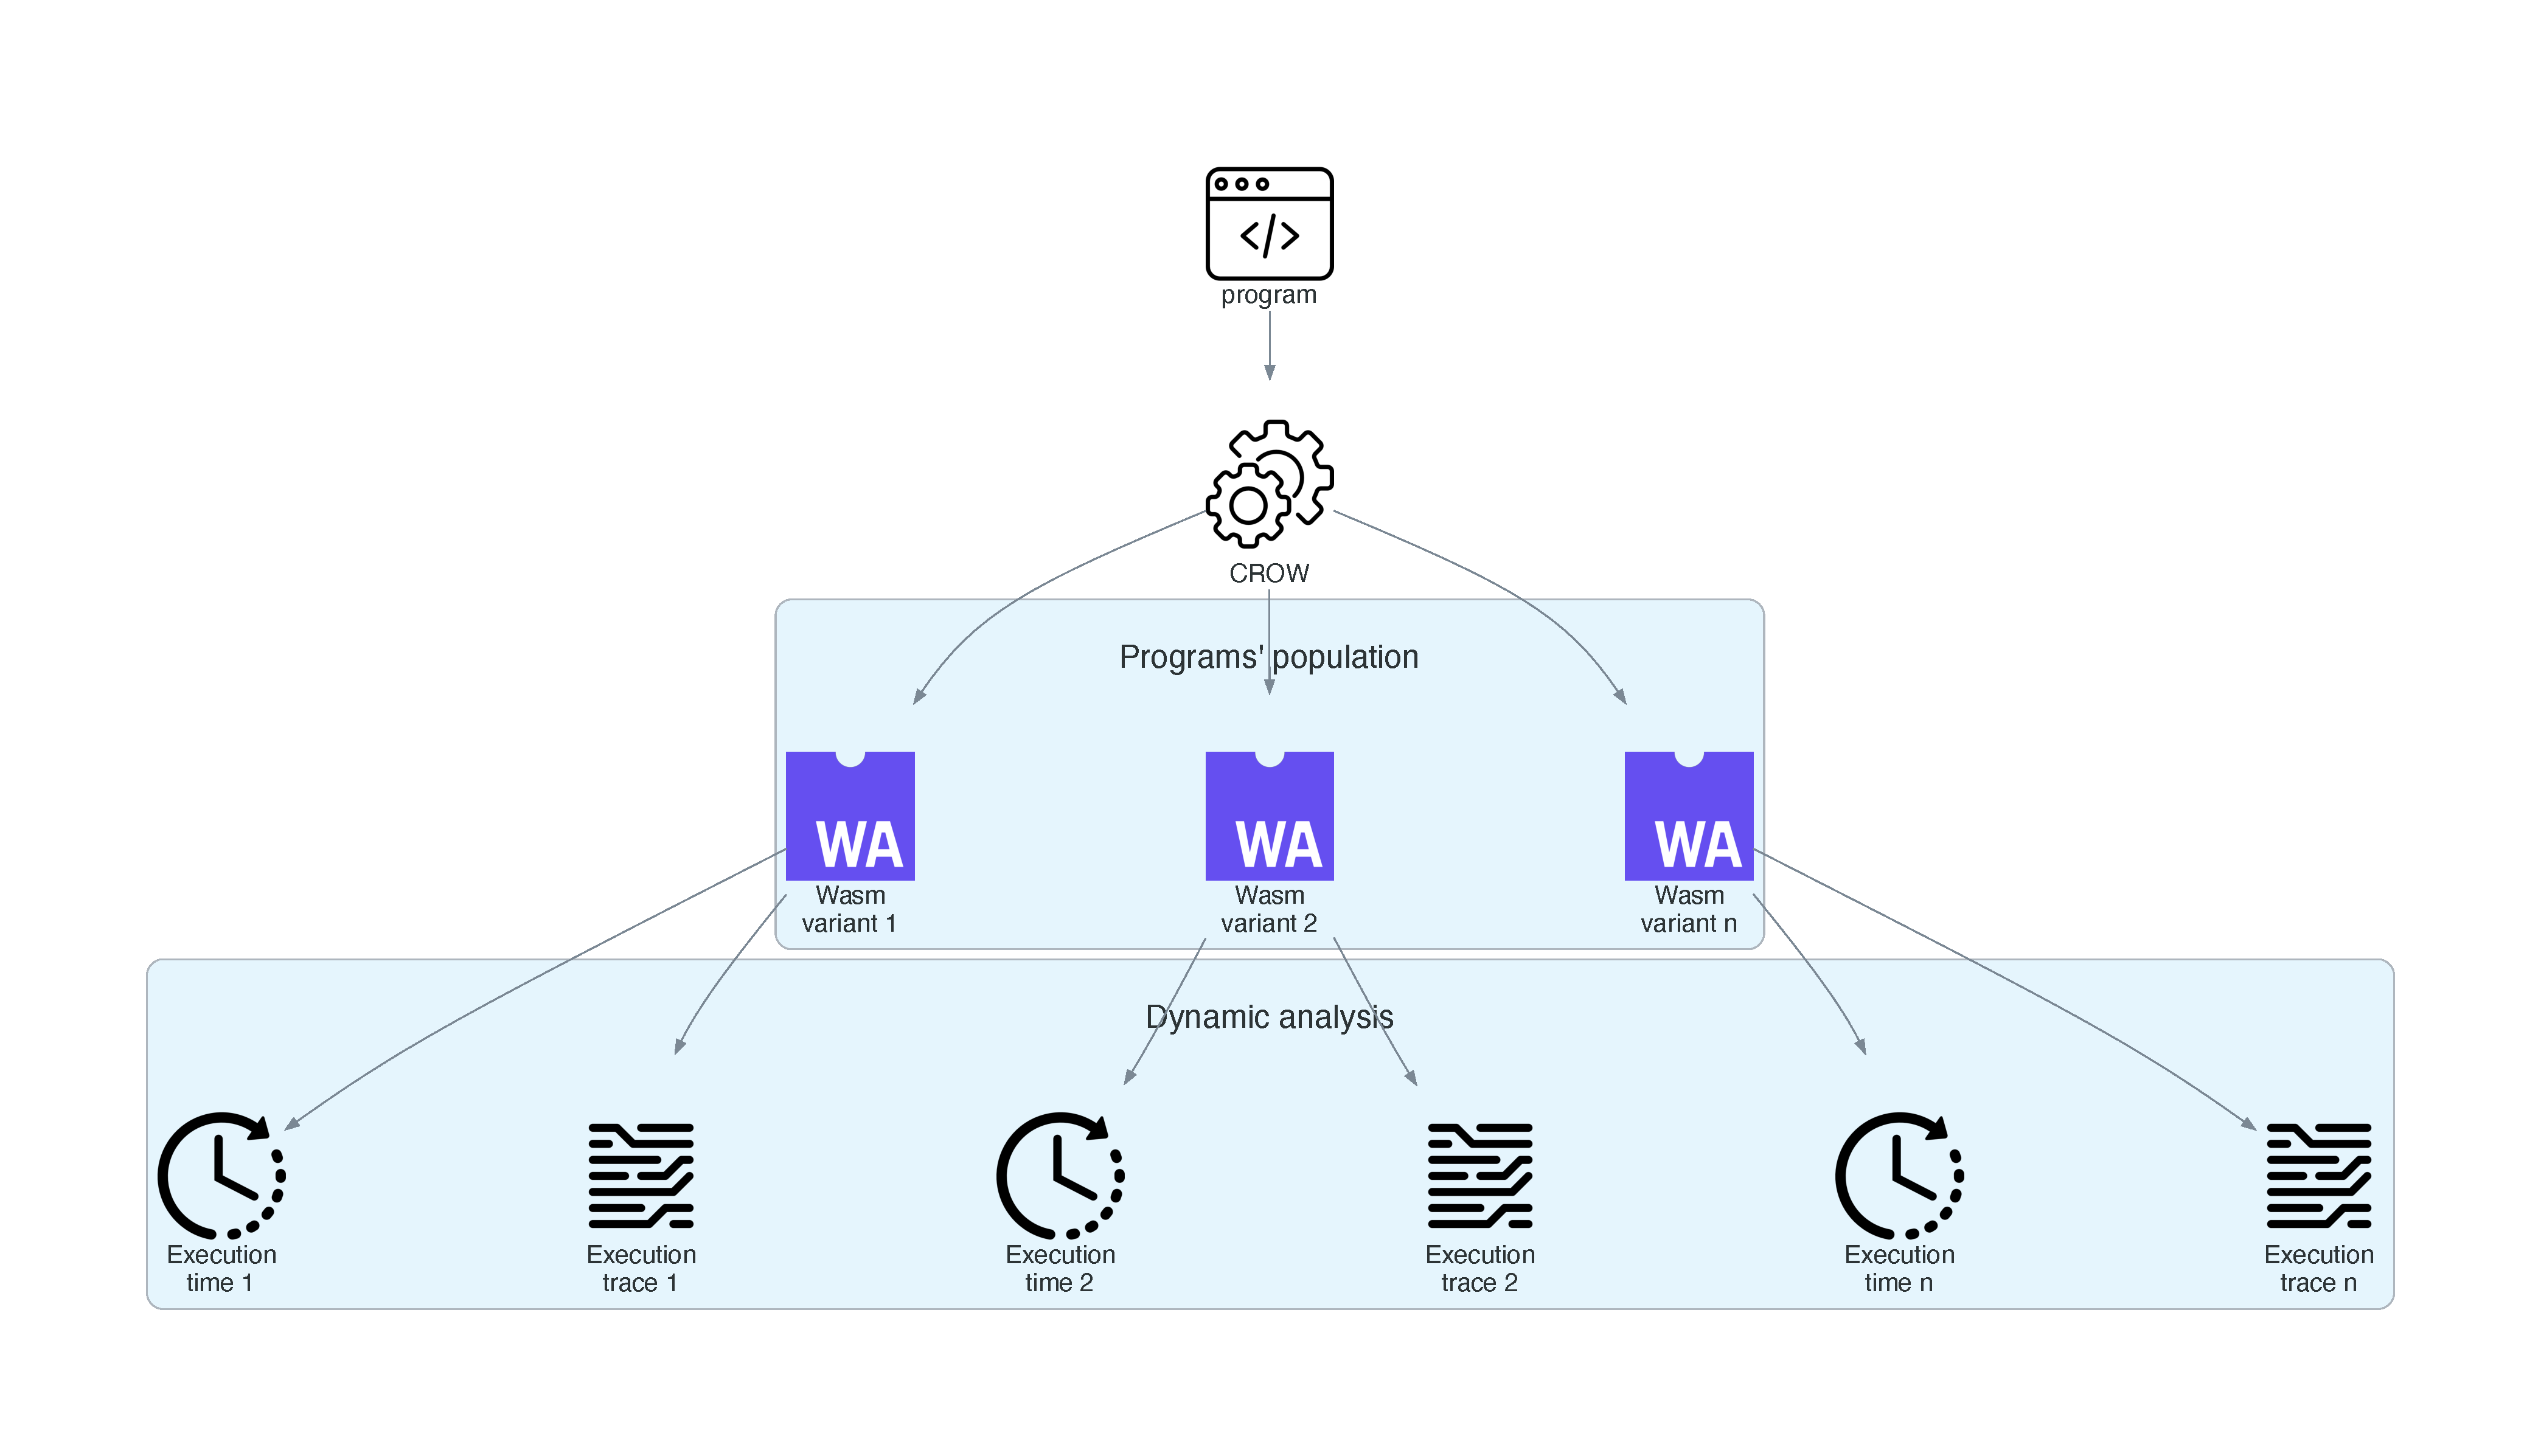
\includegraphics[width=\linewidth]{diagrams/Rq2.pdf}
    \caption{Dynamic analysis for RQ2.}
    \label{diagrams:protocol:rq2}
\end{figure*}

In this second research question, we investigate to what extent the artificially created variants are dynamically different between them and the original program. To conduct this research question, we could separate our experiments into two fields as \autoref{diagrams:protocol:rq2} illustrates: static analysis and dynamic analysis. 
The static analysis focuses on the appreciated differences among the program variants, as well as between the variants and the original program. We perform the static analysis in answering RQ1 in \autoref{rq1:method}. 
With RQ2, we focus on the last category, the dynamic analysis of the generated variants. This decision is supported because dynamic analysis complements RQ1 and, it is essential to provide a full understanding of diversification.
We use the original functions from \corpusrosetta corpus described in \autoref{section:crow:corpora} and their variants generated to answer RQ1. 
We use only \corpusrosetta to answer RQ2 because this corpus is composed of simple programs that can be executed directly without user interaction, \ie we only need to call the interpreter passing the \wasm binary to it. 
To dynamically compare programs and their variants, we execute each program on each programs' population to collect and execution times. We define execution trace and execution time in the following section.

\subsection*{Metrics}
\label{rq2:metrics}

We compare the execution traces of two any programs of the same population with a global alignment metric. We propose a global alignment approach using Dynamic Time Warping (DTW).
Dynamic Time Warping \cite{NEEDLEMAN1970443} computes the global alignment between two sequences. It returns a value capturing the cost of this alignment, which is a distance metric. The larger the DTW distance, the more different the two sequences are.
DTW has been used for comparing traces in different domains. For software, De A. Maia \etal \cite{ Maia08usinga} proposed to identify similarity between programs from execution traces.
As we discussed in \autoref{sota:wasm}, a theoretical \wasm engine perform \texttt{push} and \texttt{pop} operations when the program instructions are executed. Therefore, in our experiments, we define the execution traces as the sequence of the stack operations during the execution of the \wasm program. 
In the following, we define the $\DTW$ metric. 
 
%\todo{before, define this and give an illutrative listing plus, says how you collect those traces, that's part of the protocol: between the stack operation traces }

\begin{metric}{\DTW{}:}
\label{metric:stack}
\normalfont 
	Given two programs P and P' from the same program's population, \DTW{}(P,P'), computes the DTW distance collected during their execution. \\
	A \DTW{} of $0$ means that both traces are identical.
	The higher the value, the more different the traces. 
\end{metric}



Moreover, we use the execution time distribution of the programs in the population to complement the answer to RQ2. For each program pair in the programs' population, we compare their execution time distributions. We define the execution time as follows:

\begin{metric}{Execution time:}\label{metric:time}
    \normalfont 
	Given a \wasm program P, the execution time is the time spent to execute the binary.
\end{metric}



%\subsection{Variants preservation}

\subsection*{Protocol}

% Dynamic
To compare program and variants behavior during runtime, we analyze all the unique program variants generated to answer RQ1 in a pairwise comparison using the value of aligning their execution traces (\autoref{metric:stack}). We use SWAM\footnote{\url{https://github.com/satabin/swam}} to execute each program and variant to collect the stack operation traces. SWAM is a \wasm interpreter that provides functionalities to capture the dynamic information of \wasm program executions, including the virtual stack operations.
% \todo{Can the reader runderstand that? We want to remark that we only collect the stack operation traces due to the memory-agnosticism of our approach to generate variants. Our approach does not change the memory-like operations of the original code.}

Furthermore, we collect the execution time, \autoref{metric:time}, for all programs and their variants. We compare the collected execution time distributions between programs using a Mann-Withney U test \cite{mann1947} in a pairwise strategy.

%\todo{Maybe the first time that Mann-Withney is mentioned I should describe what it is}

 